
\begin{frame}
\frametitle{Internal Uncertainty}
\begin{itemize}
  
  \item Now that we discussed \textit{external uncertainty} over \textit{states of nature},
  let's talk about \alert{internal uncertainty}.

	\item Internal uncertainty occurs when one or more players pick their strategies randomly.

	\item Picking a strategy at random is really just a different kind of strategy, called a \alert{mixed strategy}.
\end{itemize}
\end{frame}

\begin{frame}
\frametitle{Mixed Strategies}
\begin{itemize}

	\item When a player always does the same thing, it's called a \alert{pure strategy}.
  
  \item A \alert{mixed strategy} assigns a probability to each of a player's pure strategies. 

  \begin{itemize}
    \item Like a lottery, the probabilities in a mixed strategy must all be between 0 and 1,
    \item and must sum to exactly 1.
  \end{itemize}
\end{itemize}
\end{frame}

\begin{frame}{Mixed Strategies}

\begin{itemize}

  \item A mixed strategy can assign 0 probability to a pure strategy.

  \item It can even assign probability 1 to a single pure strategy, and probability 0 to all others
  
  \begin{itemize}
    \item this is still, technically, a mixed strategy, but it is a trivial one.
  \end{itemize}

	\item When a player uses a mixed strategy, it turns the \textbf{other} player's payoffs into lotteries.
  
\end{itemize}
\end{frame}

\begin{frame}
\frametitle{Mixed Strategies in the Deer Hunt}

Consider the Deer Hunt:

\begin{table}[h]
\centering
\begin{tabular}{cc|c|c|}
	& \multicolumn{1}{c}{} & \multicolumn{2}{c}{Ogg}\\
	& \multicolumn{1}{c}{} & \multicolumn{1}{c}{$Deer$}  & \multicolumn{1}{c}{$Rabbit$} \\\cline{3-4}
	\multirow{2}*{Igg}  & $Deer$ & $2, 2$ & $0, 1$ \\\cline{3-4}
	& $Rabbit$ & $1, 0$ & $1, 1$ \\\cline{3-4}
\end{tabular}
\end{table}

\begin{itemize}
	\item Suppose that Igg hunts Deer 3/4 of the time, and Rabbit 1/4 of the time.

  \item If Ogg \textit{always hunts deer}; 
  what is Ogg's \textit{expected payoff}?

  \vspace{5mm}

	% \item Ogg's expected payoff from playing Deer will be $0.75(2) + 0.25(0) = 1.5$.
\end{itemize}
\end{frame}

\begin{frame}
\frametitle{Mixed Strategies in the Deer Hunt: Generalizing}

We can generalize this approach to calculate Ogg's expected payoffs from any strategy that Igg chooses to play:

\begin{itemize}

	\item Suppose that Igg plays Deer with probability p, and Rabbit with probability 1 - p.

	\item Then Ogg's expected payoff from Deer is:
  % $2(p) + 0(1 - p) = 2p$, and from Rabbit, it is $1(p) + 1(1 - p) = 1$.
  \vspace{20mm}

	\item Note that Ogg's expected payoff from Deer gets larger with p: the more likely Igg is to hunt Deer, the more attractive an option it becomes for Ogg.

\end{itemize}
\end{frame}

\begin{frame}
\frametitle{When to Play a Mixed Strategy?}
\begin{itemize}

	\item It's possible for a mixed strategy to be a best response to the other player's strategy:

  \begin{itemize}
    \item if and only if all of the mixed strategy's \alert{components} (pure strategies that are assigned positive probability) are best responses too.
  \end{itemize}

	\item Some intuition: If a strategy is not a best response, you should not play it---even as part of a mixed strategy.

\end{itemize}
\end{frame}

\begin{frame}{When to play a Mixed Strategy?}

  If a player only has \textbf{two pure strategies}, it becomes simple to tell when a mixed strategy is a best response: the mixed strategy must be a mixture of those two pure strategies, and the only way that both of them are best responses is if they have equal expected payoffs.

\begin{itemize}
	\item Taking the Deer Hunt as an example, the only way that it can be a best response for Ogg to play a mixed strategy is if Deer and Rabbit provide Ogg with equal expected payoffs: we must have $2p = 1$, or $p = \frac{1}{2}$.
\end{itemize}
\end{frame}

% \begin{frame}
% \frametitle{What Mixed Strategy to Play}
% \begin{itemize}
% 	\item However, if any mixed strategy is a best response, then \textbf{all} mixed strategies (with the same components) are also best responses.
% 	\item Intuitively, if the pure strategies going into a mixed strategy are just as good as each other, then it doesn't matter what proportions you mix them in.
% 	\item This means that, while it's easy to solve for \textbf{when} it's rational for a player to use a mixed strategy, there's no way to solve for a particular mixed strategy that the player \textbf{should} play.
% \end{itemize}
% \end{frame}

\begin{frame}
\frametitle{Mixed-Strategy Nash Equilibrium}
	To solve for the Nash equilibria where players are allowed to use mixed strategies:

  we need to look for the conditions under which a player would be willing to use a mixed strategy.

\begin{itemize}

	\item This means that we're going to use one player's expected payoffs to solve for the \textbf{other} player's mixed strategy

\end{itemize}
\end{frame}

\begin{frame}
\frametitle{MSNE in the Deer Hunt}
\begin{itemize}
	\item Returning to the Deer Hunt, let's say that Igg plays Deer with probability $p$ and Rabbit with probability $1 - p$...
	\item While Ogg plays Deer with probability $q$ and Rabbit with probability $1 - q$.
	\begin{itemize}
		\item This is simply a framework for describing each player's mixed strategies:
    we're using placeholder variables for the players' mixed strategy probabilities
	\end{itemize}
\end{itemize}
\end{frame}

\begin{frame}{MSNE in the Deer Hunt}
  \begin{itemize}
	\item We already saw that Ogg's expected payoffs from Deer and Rabbit are $2p$ and $1$, respectively, 
    so Ogg would only play a mixed strategy if $p = \frac{1}{2}$.

	\item Likewise, Igg's expected payoffs are $2q$ and $1$, and Igg will play a mixed strategy if $q = \frac{1}{2}$.

	\item The MSNE in this game can be written as:

    $$ \{(1/2~Deer, 1/2~Rabbit)_{Ogg}, \ (1/2~Deer, 1/2~Rabbit)_{Igg}\}$$.

\end{itemize}
\end{frame}

% \begin{frame}
% 
%   Another way to write out mixed strategies using $\sigma$:
% 
%   $$ \sigma_{Ogg} =  
% \end{frame}

\begin{frame}
\frametitle{Error-Checking}
\begin{itemize}
	\item Make sure that you're setting up the equations used to solve for a player's strategy correctly:
	\begin{itemize}
		\item Remember that you are creating an equation to describe when a player is indifferent between their pure strategies: if you're trying to figure out when \textbf{Player 1} is indifferent, you need to use \textbf{Player 1's} payoffs.
		\item However, when calculating expected payoffs, the probabilities will be based on the \textbf{other} player's mixed strategy: in a game with mixed strategies, the randomness a player deals with is created by the \textbf{other} player---not themselves.
	\end{itemize}
\end{itemize}
\end{frame}

\begin{frame}
\frametitle{Another Example: Police Patrol and Drug Trade
  \footnote{Harrington, pg. 226}}
\begin{table}[h]
	\centering
	\begin{tabular}{cc|c|c|}
		& \multicolumn{1}{c}{} & \multicolumn{2}{c}{Drug Dealer}\\
		& \multicolumn{1}{c}{} & \multicolumn{1}{c}{Streets (d)}  & \multicolumn{1}{c}{Park (1 - d)} \\\cline{3-4}
		\multirow{2}*{Police}  & Streets (p) & 80, 20 & 0,100 \\\cline{3-4}
		& Park (1 - p) & 10,90 & 60,40 \\\cline{3-4}
	\end{tabular}
\end{table}
\begin{itemize}
	\item Police Officer's expected utility:
  % $U_B(Bach) = 3q + 0(1 - q) = 3q$ and $U_B(Strav.) = 0q + 2(1 - q) = 2 - 2q$.
  \vspace{15mm}
	\item Drug Dealer's expected utility:
  % $U_S(Bach) = 2p$ and $U_S(Strav.) = 3 - 3p$.
\end{itemize}
\end{frame}

\begin{frame}{Graph Police Officer's expected utilities}
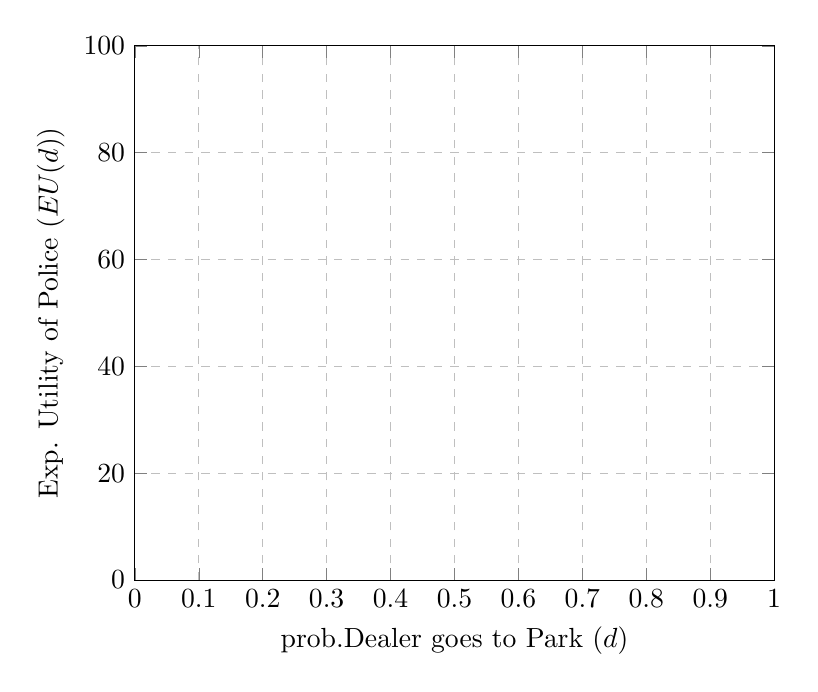
\begin{tikzpicture}
 
   \begin{axis}[
     width=0.8\textwidth,
     grid,
     xlabel={prob.Dealer goes to Park ($d$)},
     ylabel={Exp. Utility of Police ($EU(d)$)},
     xmin=0, xmax=1.0,
     ymin=0, ymax=100,
     xtick={0,.1,...,1.0},
     ytick={0,20,...,80,100},
     grid style=dashed,
     ]
 
     \addplot[draw=none] coordinates {(1,1)};
 
   \end{axis}
 \end{tikzpicture}

\end{frame}

\begin{frame}{Graph Drug Dealer's expected utilities}
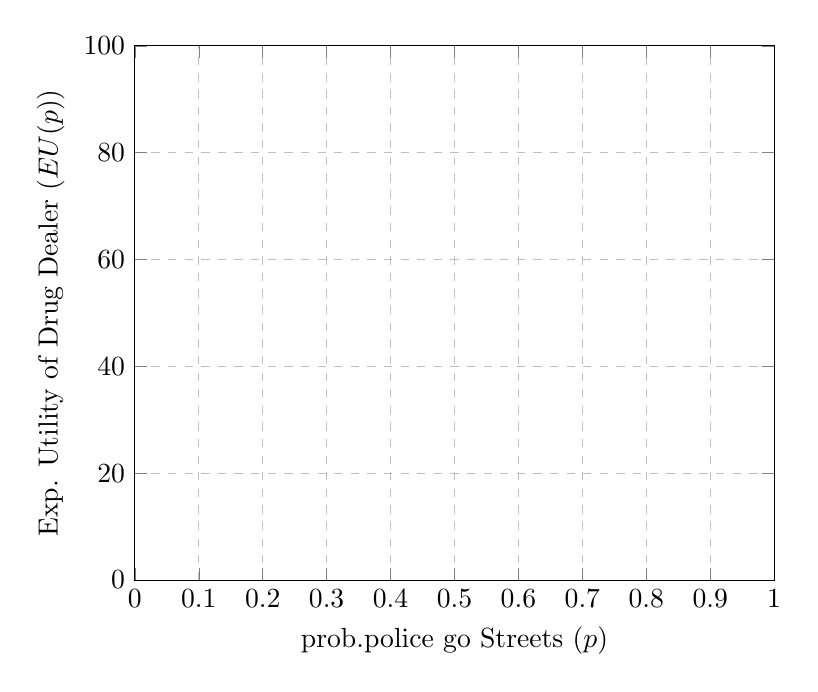
\begin{tikzpicture}
 
   \begin{axis}[
     width=0.8\textwidth,
     grid,
     xlabel={prob.police go Streets ($p$)},
     ylabel={Exp. Utility of Drug Dealer ($EU(p)$)},
     xmin=0, xmax=1.0,
     ymin=0, ymax=100,
     xtick={0,.1,...,1.0},
     ytick={0,20,...,80,100},
     grid style=dashed,
     ]
 
     \addplot[draw=none] coordinates {(1,1)};
 
   \end{axis}
 \end{tikzpicture}

\end{frame}

\begin{frame}{Graph Best Response functions}
 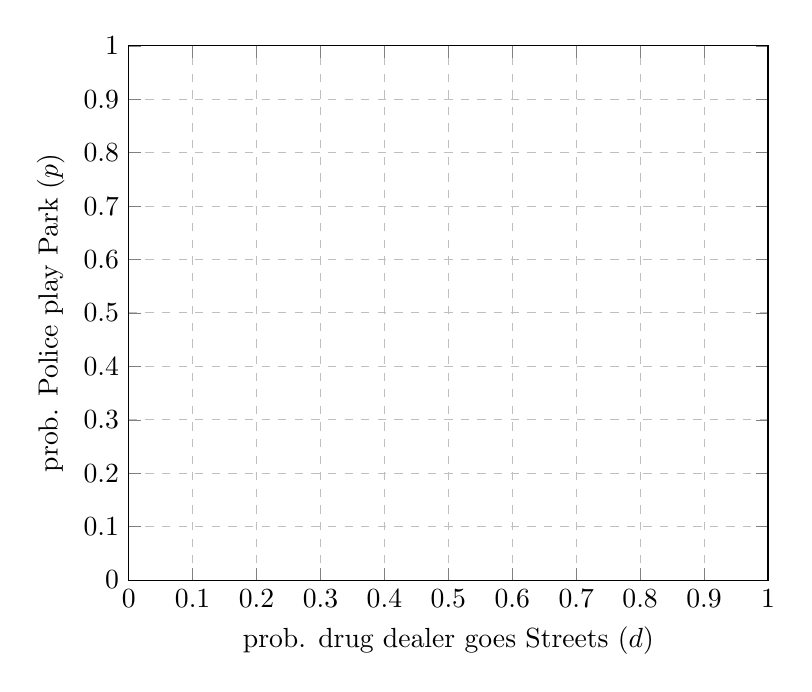
\begin{tikzpicture}
 
   \begin{axis}[
     width=0.8\textwidth,
     grid,
     xlabel={prob. drug dealer goes Streets ($d$)},
     ylabel={prob. Police play Park ($p$)},
     xmin=0, xmax=1.0,
     ymin=0, ymax=1.0,
     xtick={0,.1,...,1.0},
     ytick={0,.1,...,1.0},
     grid style=dashed,
     ]
 
     \addplot[draw=none] coordinates {(1,1)};
 
   \end{axis}
 \end{tikzpicture}
\end{frame}

\begin{frame}
\frametitle{MSNE in Patrol and Trade game:}
\begin{itemize}
\item When is the Police Officer indifferent between going to the Park and going to the Streets?
  \vspace{15mm}

\item When is the Drug Dealer indifferent between going to the Park and going to the Streets?
  \vspace{15mm}

  \item What is the \alert{Mixed Strategies Nash equilibrium?}
  \vspace{15mm}

\end{itemize}
\end{frame}

\begin{frame}{MSNE in Patrol and Trade game:}
\begin{itemize}
\item Note that the players' asymmetric preferences result in each of them buying a ticket for their more preferred concert most of the time in this MSNE.
\item If we gave them stronger preferences (i.e. increased the amount by which they prefer their favorite composer), it would amplify this effect in the MSNE.
\end{itemize}
\end{frame}

\begin{frame}
\frametitle{iClicker Q1}
\begin{itemize}
\item Consider the following game table. What are Player 1's expected payoffs, given Player 2's mixed strategy?
\end{itemize}
\begin{table}[h]
\centering
\begin{tabular}{cc|c|c|}
	& \multicolumn{1}{c}{} & \multicolumn{2}{c}{Player 2}\\
	& \multicolumn{1}{c}{} & \multicolumn{1}{c}{$Up (q)$}  & \multicolumn{1}{c}{$Down (1 - q)$} \\\cline{3-4}
	\multirow{2}*{Player 1}  & $Up (p)$ & 2, -2 & -3, 3 \\\cline{3-4}
	& $Down (1 - p)$ & -5, 5 & 1, -1 \\\cline{3-4}
\end{tabular}
\end{table}
  \begin{enumerate}[(a)]
\item $U_1(Up) = 5q - 3, U_1(Down) = 1 - 6q$
\item $U_1(Up) = 3 - 5q, U_1(Down) = 6q - 1$
\item $U_1(Up) = 5 - 7q, U_1(Down) = 1 - 6p$
\item $U_1(Up) = 7p - 5, U_1(Down) = 1 - 4p$
\item $U_1(Up) = 5 - 7p, U_1(Down) = 4p - 1$
\end{enumerate}
\end{frame}

\begin{frame}
\frametitle{iClicker Q2}
\begin{itemize}
\item Consider the following game table. What are \textbf{Player 2's} expected payoffs, given Player 1's mixed strategy?
\end{itemize}
\begin{table}[h]
\centering
\begin{tabular}{cc|c|c|}
& \multicolumn{1}{c}{} & \multicolumn{2}{c}{Player 2}\\
& \multicolumn{1}{c}{} & \multicolumn{1}{c}{$Up (q)$}  & \multicolumn{1}{c}{$Down (1 - q)$} \\\cline{3-4}
\multirow{2}*{Player 1}  & $Up (p)$ & 2, -2 & -3, 3 \\\cline{3-4}
& $Down (1 - p)$ & -5, 5 & 1, -1 \\\cline{3-4}
\end{tabular}
\end{table}
\begin{enumerate}[(a)]
\item $U_2(Up) = 5q - 3, U_2(Down) = 1 - 6q$
\item $U_2(Up) = 3 - 5q, U_2(Down) = 6q - 1$
\item $U_2(Up) = 5 - 7q, U_2(Down) = 1 - 6p$
\item $U_2(Up) = 7p - 5, U_2(Down) = 1 - 4p$
\item $U_2(Up) = 5 - 7p, U_2(Down) = 4p - 1$
\end{enumerate}
\end{frame}

\begin{frame}
\frametitle{iClicker Q3}
\begin{itemize}
\item The correct answers to the previous two questions were:
\begin{itemize}
\item $U_1(Up) = 5q - 3, U_1(Down) = 1 - 6q$.
\item $U_2(Up) = 5 - 7p, U_2(Down) = 4p - 1$.
\end{itemize}
\item Based on this, what are $p$ and $q$ in the MSNE of this game?
\begin{enumerate}[(a)]
\item $p^* = 4/11, \ q^* = 5/11$
\item $p^* = 4/11, \ q^* = 6/11$
\item $p^* = 6/11, \ q^* = 4/11$
\item $p^* = 7/11, \ q^* = 5/11$
\item $p^* = 7/11, \ q^* = 6/11$
\end{enumerate}
\end{itemize}
\end{frame}

\begin{frame}
\frametitle{An MSNE With Only One Mixed Strategy}
\begin{itemize}
	\item Consider the following game table:
\end{itemize}
\begin{table}[h]
	\centering
	\begin{tabular}{cc|c|c|}
		& \multicolumn{1}{c}{} & \multicolumn{2}{c}{Player 2}\\
		& \multicolumn{1}{c}{} & \multicolumn{1}{c}{$X~(q)$}  & \multicolumn{1}{c}{$Y~(1 - q)$} \\\cline{3-4}
		\multirow{2}*{Player 1}  & $A~(p)$ & 2, 2 & 3, 2 \\\cline{3-4}
		& $B~(1 - p)$ & 4, 3 & 0, 0 \\\cline{3-4}
	\end{tabular}
\end{table}
\begin{itemize}
	\item The players' expected payoffs are:
	\begin{itemize}
		\item $U_1(A) = 2q + 3(1 - q) = 2q + 3 - 3q = 3 - q$.
		\item $U_1(B) = 4q + 0(1 - q) = 4q$.
		\item $U_2(X) = 2p + 3(1 - p) = 2p + 3 - 3p = 3 - p$.
		\item $U_2(Y) = 2p + 0(1 - p) = 2p$.
	\end{itemize}
\end{itemize}
\end{frame}

\begin{frame}
\frametitle{An MSNE With Only One Mixed Strategy}
\begin{itemize}
\item Based on this, the conditions under which each player will use a mixed strategy are:
\end{itemize}
\begin{align*}
Player~1: && Player~2:&\\
3 - q &= 4q & 3 - p &= 2p\\
3 &= 5q & 3 &= 3p\\
q &= 3/5 & p &= 1
\end{align*}
\begin{itemize}
\item We've never seen anything like $p = 1$ in this context before...
\item $p = 1$ tells us that Player 2 will only play a mixed strategy
  if Player 1 only play A, which isn't really a mixed strategy at all.
\item This usually occurs when one strategy \textbf{weakly} dominates another.
\end{itemize}
\end{frame}

\begin{frame}
\frametitle{An MSNE With Only One Mixed Strategy}
\begin{itemize}
	\item We can still approach this the same way that we have in the past:
	\item Suppose that in the MSNE, Player 1 plays a (non-trivial) mixed strategy. Then Player 2 must also play a mixed strategy, in which q = 3/5.
	\begin{itemize}
		\item But Player 2 will only play a mixed strategy if Player 1 plays the mixed strategy where p = 1...which is a trivial mixed strategy. This is a contradiction, and it means that there is no MSNE where Player 1 plays a non-trivial mixed strategy.
	\end{itemize}
\end{itemize}
\end{frame}

\begin{frame}
\frametitle{An MSNE With Only One Mixed Strategy}
\begin{itemize}
\item Approach it the other way next: Suppose Player 2 plays a non-trivial mixed strategy. Then Player 1 must play A as a pure strategy.
\begin{itemize}
	\item Player 2 will play A if $3 - q \geq 4q$, i.e. if $3/5 \geq q$.
\end{itemize}
\item This lets Player 2 play a non-trivial mixed strategy! There is no contradiction here.
\end{itemize}
\end{frame}

\begin{frame}{An MSNE with only one mixed strategy}
\begin{itemize}
\item There are a range of MSNEs here: all strategy profiles of the form \{(1, 0), (q, 1 - q)\}, in which $q \in (0, 3/5]$, are MSNEs.
\item There are also two trivial MSNEs, \{(1, 0), (0, 1)\} and \{(0, 1), (1, 0)\}, which are really just the pure-strategy Nash equilibria (A, Y) and (B, X) expressed in the form of an MSNE.
\item It will help to understand what's going on with the Best Responses graph:
\end{itemize}
\end{frame}

\begin{frame}{Graph Best Responses}
  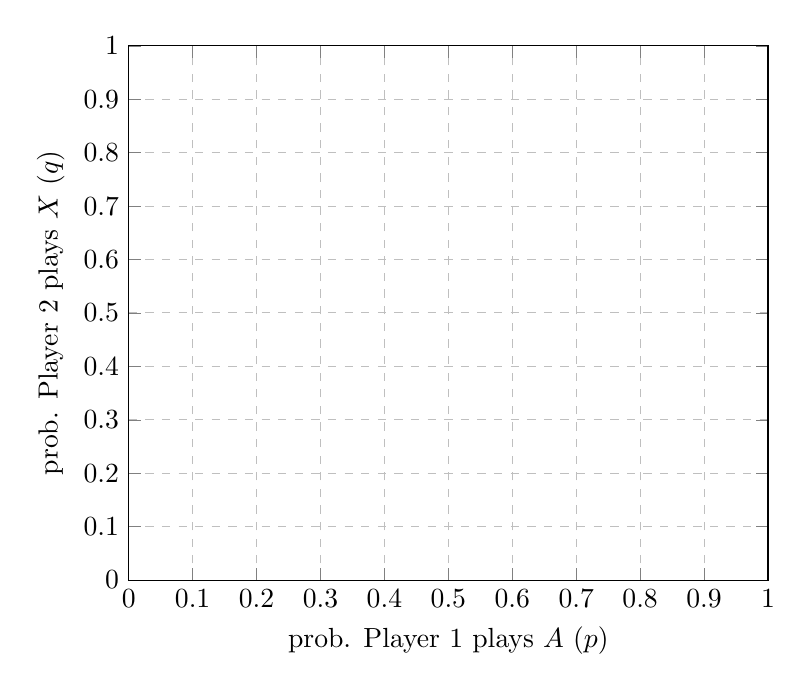
\begin{tikzpicture}
 
   \begin{axis}[
     width=0.8\textwidth,
     grid,
     xlabel={prob. Player 1 plays $A$ ($p$)},
     ylabel={prob. Player 2 plays $X$ ($q$)},
     xmin=0, xmax=1.0,
     ymin=0, ymax=1.0,
     xtick={0,.1,...,1.0},
     ytick={0,.1,...,1.0},
     grid style=dashed,
     ]
 
     \addplot[draw=none] coordinates {(1,1)};
 
   \end{axis}
 \end{tikzpicture}
 
\end{frame}

\begin{frame}
\frametitle{Absence of MSNEs}
\begin{itemize}
	\item Let us return to the Prisoner's Dilemma and check for MSNEs:
\end{itemize}
\begin{table}[h]
	\centering
	\begin{tabular}{cc|c|c|}
		& \multicolumn{1}{c}{} & \multicolumn{2}{c}{Luca}\\
		& \multicolumn{1}{c}{} & \multicolumn{1}{c}{$Testify~(q)$}  & \multicolumn{1}{c}{$Keep~Quiet~(1-q)$} \\\cline{3-4}
		\multirow{2}*{Guido}  & $Testify~(p)$ & $-10,-10$ & $0,-20$ \\\cline{3-4}
		& $Keep~Quiet~(1-p)$ & $-20,0$ & $-1,-1$ \\\cline{3-4}
	\end{tabular}
\end{table}
\begin{itemize}
	\item Guido and Luca's expected payoffs are:
	\begin{itemize}
		\item $U_G(Testify) = -10q + 0(1 - q) = -10q$.
		\item $U_G(Keep Quiet) = -20q + (-1)(1 - q) = -1 - 19q$.
		\item $U_L(Testify) = -10p + 0(1 - p) = -10p$.
		\item $U_L(Keep Quiet) = -20p + (-1)(1 - p) = -1 - 19p$.
	\end{itemize}
\end{itemize}
\end{frame}

\begin{frame}
\frametitle{Absence of MSNEs}
\begin{itemize}
\item Guido will play a mixed strategy if:
\end{itemize}
\begin{align*}
-10q &= -1 - 19q\\
9q &= -1\\
q &= -1/9
\end{align*}
\begin{itemize}
  \item But \textbf{-1/9 is not a valid probability!}
\item We could also note that if $q\in [0, 1]$, which is the range for valid probabilities, $-10q$ is always greater than $-1 - 19q$. In other words, as we saw weeks ago, $Testify$ strictly dominates $Keep~Quiet$...so why would Guido mix between the two of them?
\end{itemize}
\end{frame}

\begin{frame}
\frametitle{Getting Bad Probabilities}
\begin{itemize}
	\item If you've set up the expected-payoff equation, and solved for a player's mixed strategy, and you find that the probability is less than 0, or more than 1...
	\item \textbf{It means something is wrong.} Probability can only be between 0 and 1 (inclusive).
	\item First of all, double-check your math---it could be an algebra error.
	\item But if you're confident in your math, this means that there is \textbf{no way that the player would ever play a mixed strategy}: in fact, they have a strictly dominated strategy.
	\item There will be no MSNE where this player uses a mixed strategy---but there might be MSNEs where the other player does, so you should still check that.
\end{itemize}
\end{frame}

\begin{frame}
\frametitle{MSNE in a Larger Game}
\begin{itemize}
	\item Suppose that we have this 3$\times$2 game:
\end{itemize}
\begin{table}[h]
\centering
\begin{tabular}{cr|c|c|}
	& \multicolumn{1}{c}{} & \multicolumn{2}{c}{Player 2}\\
	& \multicolumn{1}{c}{} & \multicolumn{1}{c}{X (r)}  & \multicolumn{1}{c}{Y (1 - r)} \\\cline{3-4}
	\multirow{3}*{Player 1}  & A (p) & 2, 1 & 0, 1 \\\cline{3-4}
	& B (q) & 1, 2 & 2, 0 \\\cline{3-4}
	& C (1 - p - q) & 0, 0 & 3, 2 \\\cline{3-4}
\end{tabular}
\end{table}
\begin{itemize}
	\item First, note that in this game, Player 1's mixed strategy uses probabilities p, q, and 1 - p - q, since they have three pure strategies.
	\item As a rule of thumb, a player's mixed strategy will need one variable less than their number of strategies.
\end{itemize}
\end{frame}

\begin{frame}{Existence of Nash Equilibria}
  What is the \textit{pure strategy} Nash Equilibria of the game
  \alert{Rock, Paper, Scissors}?
\end{frame}

\begin{frame}{Existence of Nash Equilibria}
  What is the \textbf{Mixed Strategy Nash Equilibria} of the game
  \alert{Rock, Paper, Scissors}?
\end{frame}

\begin{frame}{Existence of Nash equilibria}
  Any with game with a \textit{finite} set of moves
  will have at least one \textbf{Nash equilibrium}
  when allowing for \textit{mixed strategies}.

  The true power of this concept and the most important 
  contribution of its namesake, John Nash,
  is that it is a simple concept which has universal application.
\end{frame}

\begin{frame}{Existence of Nash equilibria}
\frametitle{MSNE in a Larger Game}
\begin{itemize}
	\item To begin with, let's put together Player 1's expected payoffs, of which there will be three:
	\begin{itemize}
		\item $U_1(A) = 2r + 0 = 2r$.
		\item $U_1(B) = 1r + 2(1 - r) = 2 - r$.
		\item $U_1(C) = 0 + 3(1 - r) = 3 - 3r$.
	\end{itemize}
	\item Next, let's see what it would take to get Player 1 to mix different pairs of strategies:
	\begin{itemize}
		\item A and B: $2r = 2 - r \implies r = \frac{2}{3}$.
		\item A and C: $2r = 3 - 3r \implies r = \frac{3}{5}$.
		\item B and C: $2 - r = 3 - 3r \implies r = \frac{1}{2}$.
	\end{itemize}
	\item Note that each pair of strategies requires a different value of $r$: there is no mixed strategy for Player 2 that would make Player 1 willing to mix all three of their pure strategies.
\end{itemize}
\end{frame}

\begin{frame}
\frametitle{MSNE in a Larger Game}
\begin{itemize}
	\item Let's check Player 2's expected payoffs next:
	\begin{itemize}
		\item $U_2(X) = 1p + 2q + 0$.
		\item $U_2(Y) = 1p + 0 + 2(1 - p - q)$.
	\end{itemize}
	\item So Player 2 will play a mixed strategy if $p + 2q = p + 2(1 - p - q) \implies q = 1 - p - q$.
	\item There are two ways that this can be true: Either Player 1 plays B and C with equal probability (and we know from earlier that they would \textbf{only} be playing these two, not A), or Player 1 plays A only, and B and C not at all. 
\end{itemize}
\end{frame}

\begin{frame}
\frametitle{MSNE in a Larger Game}
\begin{itemize}
	\item So, one type of MSNE is where Player 1 only plays A: this requires $2r \geq 2 - r$ and $2r \geq 3 - 3r$, which imply that $r \geq \frac{2}{3}$ and $r \geq \frac{3}{5}$.
	\begin{itemize}
		\item MSNE: \{(1, 0, 0), (r, 1 - r)\}, where $r \geq \frac{2}{3}$.
	\end{itemize}
	\item And the other type of MSNE is where Player 1 plays B and C with equal (1/2) probability, and Player 2 plays X and Y with equal (1/2) probability.
	\begin{itemize}
		\item MSNE: \{(0, 1/2, 1/2), (1/2, 1/2)\}
	\end{itemize}
\end{itemize}
\end{frame}

